\section{Validation Exceptions}\label{code:ValidationExceptions}
In chapter \tqvref{sec:ValidationExceptions} I suggested some additional validation exceptions\index{validation exception} that are used also by the validation code described in chapter \tqfullvref{sec:CheckingMethodParametersAndReturnValues}.

The code for these exceptions is shown here. Real life implementations can be found at \autocite{TQUADRAT_ORG_FOUNDATION_NULLARGUMENTEXCEPTION} (\lstinline|NullArgumentException|\index{org.tquadrat.foundation.exception!NullArgumentException}), \autocite{TQUADRAT_ORG_FOUNDATION_EMPTYARGUMENTEXCEPTION} (\lstinline|EmptyArgumentException|\index{org.tquadrat.founcdation.exception!EmptyArgumentException}), and \autocite{TQUADRAT_ORG_FOUNDATION_BLANKARGUMENTEXCEPTION} (\lstinline|BlankArgumentException|\index{org.tquadrat.foundation.exception!BlankArgumentException}).

\begin{center}
% Generated by "dot -Tpng -y ValidationExceptions.gv > ValidationExceptions.png"
	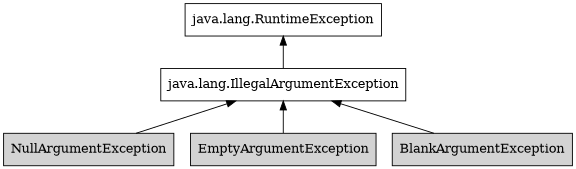
\includegraphics[scale=0.7]{code/ValidationExceptions}
\end{center}

The usage for these exception should be obvious from their names, but is also explained in the class comments.

%------------------------------------------------------------------------------

\paragraph{The Code}\
\lstinputlisting[numbers=left,caption={NullArgumentException.java}]{coding/customExceptions/NullArgumentException.java}

\lstinputlisting[numbers=left,caption={EmptyArgumentException.java}]{coding/customExceptions/EmptyArgumentException.java}

\lstinputlisting[numbers=left,caption={BlankArgumentException.java}]{coding/customExceptions/BlankArgumentException.java}

%==============================================================================
% End of file!!
%==============================================================================

